\section{Baseline Comparison}

\autoref{fig:data-terrain-evaluation-comparison} illustrates the
performance of GaitNet relative to the baseline method across a range
of terrain difficulties and commanded velocities. The results
indicate that GaitNet outperforms the baseline in most scenarios,
particularly on more challenging terrains and at higher commanded
speeds. This demonstrates the effectiveness of GaitNet in generating
robust gaits capable of adapting to varying conditions.

A closer examination of the graphs reveals that GaitNet maintains
strong performance when the commanded velocity is below 0.15\,m/s or
terrain difficulty is under 5\%. In contrast, ContactNet's
performance begins to degrade for commanded velocities above
0.05\,m/s and deteriorates further as terrain difficulty increases.
GaitNet's superior performance in these scenarios underscores the
benefits of its dynamic, acyclic gait generation capabilities.

\begin{figure}[H]
  \centering
  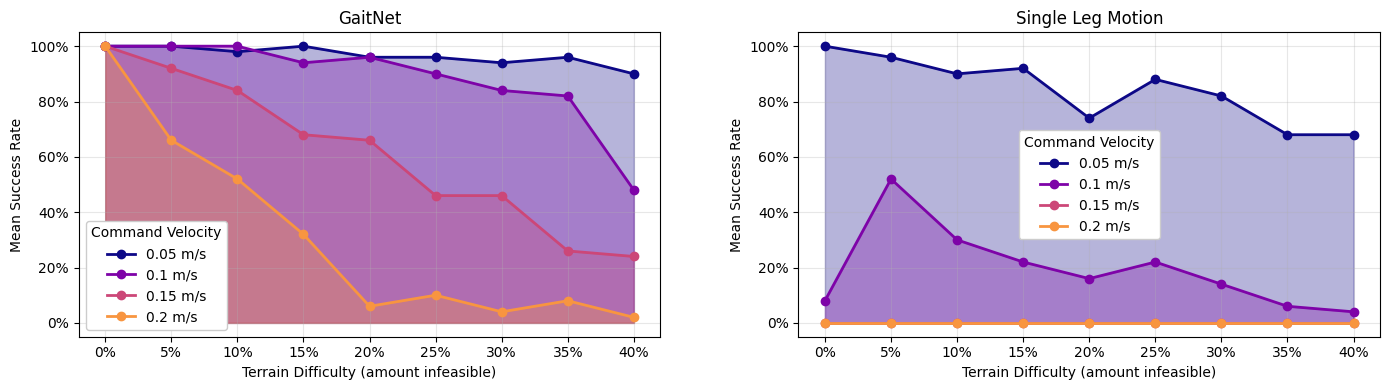
\includegraphics[width=\textwidth]{images/data/terrain-evaluation-comparison.png}
  \caption{Evaluation of GaitNet and the baseline method for
  different terrain difficulties and commanded velocities.}
  \label{fig:data-terrain-evaluation-comparison}
\end{figure}
